\section{KNTT - Lớp 11 - Ôn tập giữa học kì 1 - Đề 6}

\caulc

\Opensolutionfile{ans}[ans-ABCD]
%Câu 1
\begin{ex}%[1D1N2-2]%[KNTT - Lớp 11 - Ôn tập giữa học kì 1 - Đề 6]%[Xuan Vy Pham]
Cho góc $\alpha$ thỏa mãn $\pi<\alpha<\dfrac{3 \pi}{2}$. Chọn khẳng định đúng.
\choice
{$\sin \alpha>0$}
{$\cos \alpha>0$}
{\True $\tan \alpha>0$}
{$\cot \alpha<0$}
\loigiai
{Vì $\pi<\alpha<\dfrac{3 \pi}{2}$ nên $\sin \alpha<0$ và $\cos \alpha<0$.\\
Do đó $\tan \alpha = \dfrac{\sin \alpha}{\cos \alpha}>0$.
}
\end{ex}
%Câu 2
\begin{ex}%[1D1N2-1]%[KNTT - Lớp 11 - Ôn tập giữa học kì 1 - Đề 6]%[Xuan Vy Pham]
Chọn khẳng định đúng.
	\choice
	{$\sin \alpha + \cos \alpha =1$}
	{$\tan \alpha+ \cot \alpha =1$ $\left(\alpha \neq \dfrac{k \pi}{2}, \forall k \in \mathbb{Z}\right)$}
	{$\sin^2 \alpha \cdot \cos^2 \alpha =1$}
	{\True $\tan \alpha \cdot \cot \alpha =1$ $\left(\alpha \neq \dfrac{k \pi}{2}, \forall k \in \mathbb{Z}\right)$}
	\loigiai
	{Khẳng định đúng là $\tan \alpha \cdot \cot \alpha =1$ $\left(\alpha \neq \dfrac{k \pi}{2}, \forall k \in \mathbb{Z}\right)$.
	}
\end{ex}
%Câu 3
\begin{ex}%[1D1H1-5]%[KNTT - Lớp 11 - Ôn tập giữa học kì 1 - Đề 6]%[Xuan Vy Pham]
\immini{Trên hình vẽ, hai điểm $M$, $N$ biểu diễn các góc lượng giác có số đo là
	\choice
	{$\dfrac{\pi}{3}+k2 \pi$, $k \in \mathbb{Z}$}
	{$-\dfrac{\pi}{3}-\dfrac{k2 \pi}{3}$, $k \in \mathbb{Z}$}
	{\True $\dfrac{\pi}{3}+k \pi$, $k \in \mathbb{Z}$}
	{$\dfrac{\pi}{3}+\dfrac{k \pi}{2}$, $k \in \mathbb{Z}$}}{\begin{tikzpicture}[x=0.7cm,y=0.7cm,>=stealth,font=\footnotesize]
		\def\a{3.5}
		% Tiến hành vẽ hai trục tọa độ
		\draw[->, color=black, thick] (-\a,0) -- (\a,0) node[below] {$x$};
		\draw[->,color=black,thick] (0,-\a) -- (0,\a) node[right]{$y$};
		\draw (-0.1,0) node[above left] {$O$};
		\coordinate (O) at (0,0);
		\coordinate (A) at (\a-1,0);
		\coordinate (A') at (-\a+1,0);
		\coordinate (B) at (0,\a-1);
		\coordinate (B') at (0,-\a+1);
		\coordinate (M) at ($(O)+(60:\a-1)$);
		\coordinate (N) at ($(O)+(-120:\a-1)$);
		\draw[thick] (M)--(N);
		\draw[thick](0,0) circle (\a-1);
		\draw[thick] (0.6,0) arc (0:60:0.6) node [right] {$\tfrac{\pi}{3}$};
		\foreach \x/\g in {A/-45,A'/-135,B/50,B'/-50,M/60,N/-60}
		\fill[black] (\x) circle (1pt) ($(\g:4mm)+(\x)$) node {$\x$};	
	\end{tikzpicture}}
	\loigiai
	{Ta có $\widehat{MOA}+\widehat{AON}=\pi \Rightarrow \widehat{AON}=\pi - \dfrac{\pi}{3}=\dfrac{2 \pi}{3}$.\\
	Vì $\text{sđ}(OA,OM)=\dfrac{\pi}{3}$ và $\text{sđ}(OA,ON)=-\dfrac{2\pi}{3}=\dfrac{\pi}{3}-1 \cdot \pi$ \\
	nên $M$, $N$ là điểm biểu diễn các góc lượng giác có số đo là $\dfrac{\pi}{3}+k \pi$, $k \in \mathbb{Z}$.
	}
\end{ex}
%Câu 4
\begin{ex}%[1D1N4-3]%[KNTT - Lớp 11 - Ôn tập giữa học kì 1 - Đề 6]%[Xuan Vy Pham]
Cho đồ thị hàm số $y=\sin x$ trên đoạn $[-2 \pi;2 \pi]$. 
\begin{center}
	\begin{tikzpicture}[x=0.8cm,y=0.8 cm,>=stealth,font=\footnotesize]
		% Tiến hành vẽ hai trục tọa độ
		\draw[->, color=black, thick] (-6.8,0) -- (6.8,0) node[above] {$x$};
		\draw[->,color=black,thick] (0,-2) -- (0,2) node[right]{$y$};
		\foreach \y in 	{-1}
		\draw[shift={(0,\y)},color=black,thick] (2pt,0pt) -- (-2pt,0pt) node[below left]{$\y$};
		\foreach \y in 	{1}
		\draw[shift={(0,\y)},color=black,thick] (2pt,0pt) -- (-2pt,0pt) node[above left]{$\y$};
		\draw (-0.1,0) node[below right] {$O$};
		%Vẽ đồ thị 
		\draw[smooth, blue,thick] plot[domain=-6.28:6.28](\x,{sin((\x/(1*pi))*180)});
		\foreach \i in {-3,1}\draw [dashed]
		(0.5*pi*\i,1)--++(-90:1);
		\foreach \i in {-1,3}\draw [dashed]
		(0.5*pi*\i,0)--++(90:-1);
		\draw[dashed] (-4.71,0)--(-4.71,1)--(0,1);
		\draw[dashed] (0,-1)--(4.71,-1)--(0,-1);
		\draw (pi,0) node[below]{$\pi$};
		\draw (2*pi,0) node[below]{$2\pi$};
		\draw (-1.5*pi,0) node[below]{$\tfrac{-3 \pi}{2}$};
		\draw (-0.5*pi,0) node[above]{$\tfrac{- \pi}{2}$};
		\draw (1.5*pi,0) node[above]{$\tfrac{3\pi}{2}$};
		\draw (-pi,0) node[below]{$-\pi$};
		\draw (pi/2,0) node[below]{$\tfrac{\pi}{2}$};
		\draw (-2*pi,0) node[below]{$-2\pi$};
	\end{tikzpicture}
\end{center}
Chọn khẳng định đúng trong các khẳng định sau.
	\choice
	{\True Hàm số đồng biến trên khoảng $\left(-\dfrac{\pi}{2};\dfrac{\pi}{2}\right)$}
	{Hàm số đồng biến trên khoảng $(0;\pi)$}
	{Hàm số nghịch biến trên khoảng $(\pi;2\pi)$}
	{Hàm số nghịch biến trên khoảng $(-\pi;0)$}
	\loigiai
	{Khẳng định đúng trong các khẳng định trên là hàm số đồng biến trên khoảng $\left(-\dfrac{\pi}{2};\dfrac{\pi}{2}\right)$.
	}
\end{ex}
%Câu 5
\begin{ex}%[1D1H4-2]%[KNTT - Lớp 11 - Ôn tập giữa học kì 1 - Đề 6]%[Xuan Vy Pham]
Tập xác định của hàm số $y=\dfrac{3 \sin 2x}{1-\cos x}$ là
	\choice
	{$\mathscr{D}=\mathbb{R} \setminus \left\{k\pi, k \in \mathbb{Z}\right\}$}
	{$\mathscr{D}=\mathbb{R} \setminus \left\{1\right\}$}
	{$\mathscr{D}=\mathbb{R} \setminus \left\{\dfrac{\pi}{2}+k2\pi, k \in \mathbb{Z}\right\}$}
	{\True$\mathscr{D}=\mathbb{R} \setminus \left\{k2\pi, k \in \mathbb{Z}\right\}$}
	\loigiai
	{$y$ xác định $\Leftrightarrow 1-\cos x \neq 0 \Leftrightarrow \cos x \neq 1 \Leftrightarrow x \neq k 2\pi$, $k \in \mathbb{Z}$.\\
	Vậy $\mathscr{D}=\mathbb{R} \setminus \left\{k 2 \pi, k \in \mathbb{Z}\right\}$.
	}
\end{ex}
%Câu 6
\begin{ex}%[1D1H5-3]%[KNTT - Lớp 11 - Ôn tập giữa học kì 1 - Đề 6]%[Xuan Vy Pham]
Cho đồ thị hàm số $y=\cos x$. 
\begin{center}
		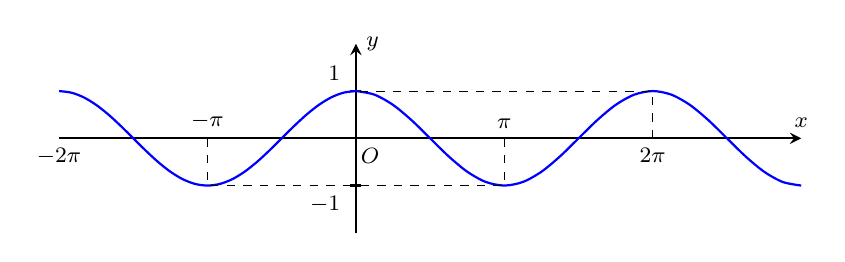
\begin{tikzpicture}[x=0.6cm,y=0.6 cm,>=stealth,font=\footnotesize]
			% Tiến hành vẽ hai trục tọa độ
			\draw[->, color=black, thick] (-2*pi,0) -- (3*pi,0) node[above] {$x$};
			\draw[->,color=black,thick] (0,-2) -- (0,2) node[right]{$y$};
			\foreach \y in 	{-1}
			\draw[shift={(0,\y)},color=black,thick] (2pt,0pt) -- (-2pt,0pt) node[below left]{$\y$};
			\foreach \y in 	{1}
			\draw[shift={(0,\y)},color=black,thick] (2pt,0pt) -- (-2pt,0pt) node[above left]{$\y$};
			\draw (-0.1,0) node[below right] {$O$};
			%Vẽ đồ thị 
			\draw[smooth, blue,thick] plot[domain=-2*pi:0](\x,{cos((\x/(1*pi))*180)});
			\draw[smooth, blue,thick] plot[domain=0:3*pi](\x,{cos((\x/(1*pi))*180)});
			\draw[dashed] (-pi,0)--(-pi,-1)--(0,-1);
			\draw[dashed] (pi,0)--(pi,-1)--(0,-1);
			\draw[dashed] (2*pi,0)--(2*pi,1)--(0,1);
			\draw (pi,0) node[above]{$\pi$};
			\draw (2*pi,0) node[below]{$2\pi$};
			\draw (-pi,0) node[above]{$-\pi$};
			\draw (-2*pi,0) node[below]{$-2\pi$};
		\end{tikzpicture}
\end{center}
Số nghiệm của phương trình $2 \cos x-1=0$ trên đoạn $[-\pi;2\pi]$ là
	\choice
	{$1$}
	{\True $3$}
	{$2$}
	{$4$}
	\loigiai
	{Ta có $2 \cos x -1 = 0 \Leftrightarrow \cos x =\dfrac{1}{2}$.\\
	Đường thẳng $y=\dfrac{1}{2}$ cắt đồ thị hàm số $y=\cos x$ trên đoạn $[-\pi;2\pi]$ tại $3$ điểm \\
	nên số nghiệm của phương trình $\cos x =\dfrac{1}{2}$ trên đoạn $[-\pi;2\pi]$ là $3$.
	}
\end{ex}
%Câu 7
\begin{ex}%[1D2N2-4]%[KNTT - Lớp 11 - Ôn tập giữa học kì 1 - Đề 6]%[Xuan Vy Pham]
Cho cấp số cộng $(u_n)$ với số hạng đầu là $u_1=15$ và công sai $d=-2$. Số hạng thứ $8$ bằng 
	\choice
	{\True $1$}
	{$-1$}
	{$103$}
	{$64$}
	\loigiai
	{Số hạng thứ $8$ là $u_8=u_1+7d=15+7 \cdot (-2)=1$.
	}
\end{ex}
%Câu 8
\begin{ex}%[1D2H2-4]%[KNTT - Lớp 11 - Ôn tập giữa học kì 1 - Đề 6]%[Xuan Vy Pham]
Cho cấp số cộng $(u_n)$ được xác định bởi $\heva{&u_1=2\\&u_{n+1}=u_n+3,n \ge 1}$. Tìm số hạng thứ $20$ của dãy số $(u_n)$?
	\choice
	{\True $59$}
	{$60$}
	{$58$}
	{$57$}
	\loigiai
	{Ta có $u_{n+1}-u_n=3$, $\forall n \in \mathbb{N}^*$.\\
	Do đó $(u_n)$ là cấp số cộng có $u_1=2$ và $d=3$.\\
	Số hạng thứ $20$ là $u_{20}=u_1+19d=2+19 \cdot 3 =59$.
	}
\end{ex}
%Câu 9
\begin{ex}%[1H4N1-3]%[KNTT - Lớp 11 - Ôn tập giữa học kì 1 - Đề 6]%[Xuan Vy Pham]
Cho hình chóp $S.ABCD$ với $ABCD$ là hình bình hành tâm $O$. Khi đó giao tuyến của hai mặt phẳng $(SAC)$ và $(SBD)$ là
	\choice
	{đường thẳng $SC$}
	{đường thẳng $SB$}
	{đường thẳng $SD$}
	{\True đường thẳng $SO$}
	\loigiai
	{\begin{center}
			\begin{tikzpicture}[line join=round, line cap=round,>=stealth,font=\footnotesize,scale=1]
				\def\a{3}
				\def\b{2}
				\def\h{3}
				\path 	(0:0) coordinate (A)
				++(0:\a) coordinate (D)
				++(-130:\b) coordinate (C)
				($(A)+(C)-(D)$) coordinate (B)
				($(A)+(80:\h)$) coordinate (S)
				($(A)!1/2!(C)$) coordinate (O);
				\draw[dashed,thick] (S)--(A)--(B) (D)--(A) (A)--(C) (B)--(D);
				\draw[thick] (S)--(B)--(C)--(D)--(S)--(C);
				\foreach \x/\g in {A/180,B/180,C/0,D/0,S/180,O/-90}
				\fill[black] (\x) circle (1pt) ($(\g:4mm)+(\x)$) node {$\x$};	
			\end{tikzpicture}
		\end{center}
	$\heva{&S \in (SAC)\\&S \in (SBD)} \Rightarrow S \in (SAC) \cap (SBD)$. (1)\\
	$\heva{&O \in AC, \; AC \subset (SAC) \\ &O \in BD, \; BD \subset (SBD)} \Rightarrow O \in (SAC) \cap (SBD)$. (2)\\
	Từ (1) và (2) suy ra $(SAC) \cap (SBD)=SO$.
	}
\end{ex}
%Câu 10
\begin{ex}%[1H4H4-2]%[KNTT - Lớp 11 - Ôn tập giữa học kì 1 - Đề 6]%[Xuan Vy Pham]
Cho hình chóp $S.ABCD$ có đáy là hình bình hành. Gọi $M$, $N$, $P$ lần lượt là trung điểm của $AB$, $BC$, $SB$. Mặt phẳng $(MNP)$ song song với mặt phẳng nào dưới đây?
	\choice
	{$(ABCD)$}
	{$(SAB)$}
	{$(SAD)$}
	{\True $(SAC)$}
	\loigiai
	{	\begin{center}
			\begin{tikzpicture}[line join=round, line cap=round,>=stealth,font=\footnotesize,scale=1]
			\def\a{3}
			\def\b{2.8}
			\def\h{3.4}
			\path 	(0:0) coordinate (A)
			++(0:\a) coordinate (D)
			++(-140:\b) coordinate (C)
			($(A)+(C)-(D)$) coordinate (B)
			($(A)+(70:\h)$) coordinate (S)
			($(A)!1/2!(B)$) coordinate (M)
			($(B)!1/2!(C)$) coordinate (N)
			($(S)!1/2!(B)$) coordinate (P);
			\draw[dashed,thick] (S)--(A)--(B) (D)--(A) (A)--(C)  (P)--(M)--(N);
			\draw[thick] (S)--(B)--(C)--(D)--(S)--(C) (N)--(P);
			\foreach \x/\g in {A/40,B/180,C/0,D/0,S/180,M/-100,N/-90,P/140}
			\fill[black] (\x) circle (1pt) ($(\g:4mm)+(\x)$) node {$\x$};	
		\end{tikzpicture}
		\end{center}
		Xét tam giác $ABC$ có $M$, $N$ lần lượt là trung điểm của $AB$, $BC$\\
		nên $MN$ là đường trung bình của $\Delta ABC$.
		Do đó $MN \parallel AC$.\\
		Ta có $\heva{&MN \parallel AC\\&AC \subset (SAC)\\&MN \not \subset (SAC) } \Rightarrow MN \parallel (SAC)$.\\
		Xét tam giác $SAB$ có $M$, $P$ lần lượt là trung điểm của $AB$, $SB$\\
		nên $MP$ là đường trung bình của $\Delta SAB$.
		Do đó $MP \parallel SA$.\\
		Ta có $\heva{&MP \parallel SA\\&SA \subset (SAC)\\&MP \not \subset (SAC) } \Rightarrow MP \parallel (SAC)$.\\
		Ta có $\heva{&MN \parallel (SAC)\\&MP \parallel (SAC) \\&\text{Trong $(MNP)$, $MN \cap MP=M$}\\
		} \Rightarrow (MNP) \parallel (SAC)$.
}
\end{ex}
%Câu 11
\begin{ex}%[1H4H4-4]%[KNTT - Lớp 11 - Ôn tập giữa học kì 1 - Đề 6]%[Xuan Vy Pham]
Cho hình chóp $S.ABCD$ có đáy là hình thang đáy lớn $AD$ gấp đôi đáy bé $BC$. Gọi $M$ là trung điểm của $CD$, $G$ là trọng tâm tam giác $ACD$, $O$ là giao điểm của $AC$ và $BD$. Đường thẳng $OG$ song song với mặt phẳng nào dưới đây
	\choice
	{$(ABCD)$}
	{$(SAB)$}
	{$(SAD)$}
	{\True $(SCD)$}
	\loigiai
	{\begin{center}
			\begin{tikzpicture}[line join=round, line cap=round,>=stealth,font=\footnotesize,scale=1]
				\def\a{4.6}
				\def\b{2.8}
				\def\h{3.4}
				\path 	(0:0) coordinate (A)
				++(0:\a) coordinate (D)
				(A)++(-50:\b) coordinate (B)
				++(0:\a/2) coordinate (C)
				($(A)+(70:\h)$) coordinate (S)
				($(C)!1/2!(D)$) coordinate (M)
				($(A)!2/3!(M)$) coordinate (G)
				($(A)!2/3!(C)$) coordinate (O)
			;
				\draw[dashed,thick] (A)--(D)(A)--(M) (A)--(C) (B)--(D) (O)--(G);
				\draw[thick] (S)--(A)--(B)--(C)--(D)--(S)--(B) (S)--(C);
				\foreach \x/\g in {A/180,B/180,C/0,D/0,S/180,M/0,G/110,O/-90}
				\fill[black] (\x) circle (1pt) ($(\g:4mm)+(\x)$) node {$\x$};	
			\end{tikzpicture}
		\end{center}
		Vì $G$ là trọng tâm $\triangle ACD$ và $M$ là trung điểm $CD$ nên $G \in AM$ và $\dfrac{AG}{AM}=\dfrac{2}{3}$.\\
		Theo định lý Thales, ta có $\dfrac{AO}{OC}=\dfrac{AD}{BC}=2$ (do $AD$ gấp đôi $BC$).\\
		Suy ra $\dfrac{AO}{AC}=\dfrac{2}{3}$.\\
		Xét tam giác $ACM$ có $\heva{&O \in AC, \; G \in AM\\&\dfrac{AO}{AC}=\dfrac{AG}{AM}=\dfrac{2}{3}} \Rightarrow OG \parallel MC$.\\
		Mà $M \in CD$ nên $OG \parallel CD$.\\
		Ta có $\heva{&OG \parallel CD\\&CD \subset (SCD)\\&OG \not\subset (SCD)} \Rightarrow OG\parallel (SCD)$.
	}
\end{ex}
%Câu 12
\begin{ex}%[1H4H2-2]%[KNTT - Lớp 11 - Ôn tập giữa học kì 1 - Đề 6]%[Xuan Vy Pham]
Cho tứ diện $ABCD$, gọi $G_1$, $G_2$ lần lượt là trọng tâm của tam giác $BCD$ và $ACD$. Tìm tỉ số $\dfrac{G_1G_2}{AB}$.
	\choice
	{$\dfrac{G_1G_2}{AB}=\dfrac{1}{2}$}
	{$\dfrac{G_1G_2}{AB}=2$}
	{$\dfrac{G_1G_2}{AB}=\dfrac{2}{3}$}
	{\True $\dfrac{G_1G_2}{AB}=\dfrac{1}{3}$}
	\loigiai
	{\begin{center}
			\begin{tikzpicture}[line join=round, line cap=round,>=stealth,font=\footnotesize,scale=1]
				\def\a{4}
				\def\b{2}
				\def\h{3.3}
				\path (0:0) coordinate (B)
				++(0:\a) coordinate (D)
				(B)++(-60:\b) coordinate (C)
				($(A)+(70:\h)$) coordinate (A)
				($(D)!1/2!(C)$) coordinate (M)
				($(B)!2/3!(M)$) coordinate (G_1)
				($(A)!2/3!(M)$) coordinate (G_2);
				\draw[dashed,thick] (B)--(D) (B)--(M) (G_1)--(G_2);
				\draw[thick] (A)--(B)--(C)--(D)--(A)--(C) (A)--(M);
				\foreach \x/\g in {B/180,C/-90,D/0,A/180,M/-90,G_1/-90,G_2/0}
				\fill[black] (\x) circle (1pt) ($(\g:4mm)+(\x)$) node {$\x$};	
			\end{tikzpicture}
		\end{center}
	Gọi $M$ là trung điểm $CD$.\\
	Xét $\triangle ABM$ có $G_1$, $G_2$ lần lượt là trọng tâm của $\triangle BCD$, $\triangle ACD$\\
	nên $\heva{&G_1 \in BM, \; G_2 \in AM\\&\dfrac{MG_1}{MB}=\dfrac{MG_2}{MA}=\dfrac{1}{3}}$.\\
	Do đó theo định lý Thales đảo, ta được $G_1 G_2 \parallel AB$.\\
	Theo định lý Thales, ta có $\dfrac{G_1G_2}{AB}=\dfrac{MG_1}{MB}=\dfrac{1}{3}$.
	}
\end{ex}
\Closesolutionfile{ans}

\indapan{6}{ans-ABCD}

\cauds

\Opensolutionfile{ans}[ans-DS]
%Câu 13
\begin{ex}%[1D1H5-1]%[KNTT - Lớp 11 - Ôn tập giữa học kì 1 - Đề 6]%[Xuan Vy Pham]
Cho hai hàm số $f(x)=\sin 2x$ và $g(x)=\cos x$.
\choiceTF
{\True Tập xác định của hàm số $f(x)$ là $\mathscr{D}=\mathbb{R}$}
{Hàm số $f(x)$ là hàm số chẵn}
{\True Hàm số $f(x)$ là hàm số tuần hoàn với chu kỳ $T=\pi$}
{$f(x)=0$ và $g(x)=0$ là hai phương trình tương đương}
\loigiai
{
% Lời giải chung
\begin{itemchoice}
\itemch Đúng. Vì hàm số $f(x)=\sin 2x$ có tập xác định là $\mathscr{D}=\mathbb{R}$.
\itemch Sai. Với mọi $x \in \mathbb{R}$, ta có
$$f(-x)=\sin(-2x)=-\sin2x=-f(x).$$
Do đó $f(x)$ là hàm số lẻ.
\itemch Đúng. Hàm số $f(x)=\sin 2x$ là hàm số tuần hoàn với chu kỳ $T=\pi$.
\itemch Sai. \\
Ta có $f(x)=0 \Leftrightarrow \sin 2x=0 \Leftrightarrow 2x = k \pi (k \in \mathbb{Z}) \Leftrightarrow x =\dfrac{k \pi}{2}(k \in \mathbb{Z})$.\\
Do đó phương trình $f(x)=0$ có tập nghiệm là $S_1=\left\{\dfrac{k \pi}{2} \mid k \in \mathbb{Z}\right\}$.\\
Ta có $g(x)=0 \Leftrightarrow \cos x =0 \Leftrightarrow x =\dfrac{\pi}{2} + k \pi (k \in \mathbb{Z})$.\\
Do đó phương trình $g(x)=0$ có tập nghiệm là $S_2=\left\{\dfrac{\pi}{2}+k \pi \mid k \in \mathbb{Z}\right\}$.\\
Xét $S_1=\left\{\dfrac{k \pi}{2} \mid k \in \mathbb{Z}\right\}$ và $S_2=\left\{\dfrac{\pi}{2}+k \pi \mid k \in \mathbb{Z}\right\}$.\\
Vì $\pi=\dfrac{2\pi}{2}$ nên $\pi \in S_1$.\\
Giả sử $\pi \in S_2$. Khi đó $\pi=\dfrac{\pi}{2}+k \pi$ với $k \in \mathbb{Z}$.\\
Ta có $\pi=\dfrac{\pi}{2}+k \pi \Leftrightarrow 1=\dfrac{1}{2}+k \Leftrightarrow k =\dfrac{1}{2}$ (vô lý vì $k \in \mathbb{Z}$).\\
Vậy $\pi \in S_1$ và $\pi \notin S_2$.\\
Nên $S_1$ và $S_2$ không là hai tập hợp bằng nhau suy ra $f(x)=0$ và $g(x)=0$ không là hai phương trình tương đương.
\end{itemchoice}
}
\end{ex}
%Câu 14
\begin{ex}%[1D2H2-6]%[KNTT - Lớp 11 - Ôn tập giữa học kì 1 - Đề 6]%[Xuan Vy Pham]
Cho dãy số $(u_n)$ với $u_n=3n-1$.
	\choiceTF
	{Dãy số $(u_n)$ là dãy số giảm}
	{\True Dãy số $(u_n)$ là một cấp số cộng với $u_1=2$ và $d=3$}
	{\True Số $179$ là số hạng thứ $60$ của dãy số $(u_n)$}
	{Biết $S_n=5430$. Khi đó $n=59$}
	\loigiai
	{
		% Lời giải chung
		\begin{itemchoice}
			\itemch Sai.\\ Với mọi $n \in \mathbb{N}^*$, ta có\\ $u_{n+1}-u_n=3(n+1)-1-(3n-1)=3n+3-1-3n+1=3>0$.\\
			Do đó $(u_n)$ là dãy số tăng.
			\itemch Đúng. Vì $u_{n+1}-u_n=3$, $\forall n \in \mathbb{N}^*$ nên $(u_n)$ là cấp số cộng với $u_1=2$ và $d=3$.
			\itemch Đúng. \\
			Giả sử số $179$ là số hạng thứ $n$ của cấp số cộng $(u_n)$.\\
			Do đó $u_n = 179 \Rightarrow u_1+(n-1)d=179 \Rightarrow 2+3(n-1)=179 \Rightarrow n=60$.\\
			Vậy số $179$ là số hạng thứ $60$ của dãy số $(u_n)$.
			\itemch Sai. \begin{align*}
				S_n=5430&\Leftrightarrow \dfrac{n[2u_1+(n-1)d]}{2} = 5430\\
				&\Leftrightarrow \dfrac{n[2 \cdot 2 +3(n-1)]}{2}=540\\
				&\Leftrightarrow \dfrac{4n+3n(n-1)}{2}=5430\\
				&\Leftrightarrow 3n^2+n-10860=0\\
				&\Leftrightarrow \hoac{&n=60\\&n=-\dfrac{181}{3}\; (\text{loại vì $n \in \mathbb{N}^*$}).}
			\end{align*}
			Vậy $n=60$.
		\end{itemchoice}
	}
\end{ex}
%Câu 15
\begin{ex}%[1D1H5-5]%[KNTT - Lớp 11 - Ôn tập giữa học kì 1 - Đề 6]%[Xuan Vy Pham]
Cho hai phương trình $\sin x=0$ và $\cos \left(2x-\dfrac{\pi}{3}\right)=1$.
	\choiceTF
	{Tập nghiệm của phương trình $\sin x=0$ là $S=\left\{k2\pi \mid k \in \mathbb{Z}\right\}$}
	{\True Tập nghiệm của phương trình $\cos \left(2x-\dfrac{\pi}{3}\right)=1$ là $S=\left\{\dfrac{\pi}{6}+k\pi \mid k \in \mathbb{Z}\right\}$}
	{Số nghiệm của phương trình $\sin x=0$ trên $[0;2\pi]$ là $2$}
	{\True Tập nghiệm của phương trình $\cos \left(2x-\dfrac{\pi}{3}\right)=\sin x$ là\\ $S=\left\{-\dfrac{\pi}{6}+k2\pi; \dfrac{5 \pi}{18}+\dfrac{k 2 \pi}{3} \mid k \in \mathbb{Z}\right\}$}
	\loigiai
	{
		% Lời giải chung
		\begin{itemchoice}
			\itemch Sai. Ta có
			$\sin x = 0 \Leftrightarrow x = k \pi (k \in \mathbb{Z})$.\\
			Vậy tập nghiệm của phương trình $\sin x=0$ là $S=\left\{k\pi \mid k \in \mathbb{Z}\right\}$.
			\itemch Đúng. Ta có\\
			$\cos \left(2x-\dfrac{\pi}{3}\right)=1 \Leftrightarrow 2x-\dfrac{\pi}{3}= k2 \pi (k \in \mathbb{Z}) \Leftrightarrow x = \dfrac{\pi}{6}+k \pi (k \in \mathbb{Z}).$\\
			Vậy tập nghiệm của phương trình $\cos \left(2x-\dfrac{\pi}{3}\right)=1$ là $S=\left\{\dfrac{\pi}{6}+k\pi \mid k \in \mathbb{Z}\right\}$
			\itemch Sai.\\
			Ta có $\sin x =0 \Leftrightarrow x = k \pi (k \in \mathbb{Z})$.\\
			Xét trên đoạn $[0;2\pi]$, ta có\\
			$x \in [0;2\pi] \Rightarrow 0 \le x \le 2 \pi \Rightarrow 0 \le k \pi \le 2 \pi \Rightarrow 0 \le k \le 2$.\\
			Mà $k \in \mathbb{Z}$ nên $k \in \left\{0;1;2\right\}$.\\
			Với $k=0 \Rightarrow x =0$.\\
			Với $k=1 \Rightarrow x = \pi$.\\
			Với $k=2 \Rightarrow x=2 \pi$.\\
			Vậy tập các nghiệm của phương trình $\sin x=0$ trên $[0;2\pi]$ là $\left\{0;\pi;2\pi\right\}$.\\
			Do đó số nghiệm cần tìm là $3$.
			\itemch Đúng. Ta có
			\allowdisplaybreaks
			\begin{align*}
				\cos \left(2x-\dfrac{\pi}{3}\right)=\sin x &\Leftrightarrow 	\cos \left(2x-\dfrac{\pi}{3}\right)=\cos \left(\dfrac{\pi}{2}-x\right) \\
				&\Leftrightarrow \hoac{&2x-\dfrac{\pi}{3}=\dfrac{\pi}{2}-x + k 2 \pi \\&2x-\dfrac{\pi}{3} = -\left(\dfrac{\pi}{2}-x\right)+k 2 \pi} (k \in \mathbb{Z}) \\
				&\Leftrightarrow \hoac{&3x=\dfrac{5\pi}{6}+ k 2 \pi \\&x = -\dfrac{\pi}{6}+k 2 \pi} (k \in \mathbb{Z}) \\
				&\Leftrightarrow \hoac{&x=\dfrac{5\pi}{18}+ \dfrac{k 2 \pi}{3} \\&x = -\dfrac{\pi}{6}+k 2 \pi} (k \in \mathbb{Z}).
			\end{align*}
			Vậy tập nghiệm $S$ của phương trình $\cos \left(2x-\dfrac{\pi}{3}\right)=\sin x$ là $\left\{-\dfrac{\pi}{6}+k2\pi; \dfrac{5 \pi}{18}+\dfrac{k 2 \pi}{3} \mid k \in \mathbb{Z}\right\}$.
		\end{itemchoice}
	}
\end{ex}
%Câu 16
\begin{ex}%[1H4H3-2]%[KNTT - Lớp 11 - Ôn tập giữa học kì 1 - Đề 6]%[Xuan Vy Pham]
Cho hình chóp $S.ABCD$ có đáy là hình bình hành tâm $O$. Gọi $M$ là trung điểm của $SC$ và $I$ là giao điểm của $AM$ với $SO$.
	\choiceTF
	{\True Đường thẳng $OM$ song song với mặt phẳng $(SAB)$}
	{\True Giao tuyến của hai mặt phẳng $(SBD)$ và mặt phẳng $(SAC)$ là đường thẳng $SO$}
	{\True Giao điểm của đường thẳng $AM$ với $(SBD)$ là $I$}
	{$IA=IM$}
	\loigiai
	{\begin{center}
			\begin{tikzpicture}[line join=round, line cap=round,>=stealth,font=\footnotesize,scale=1]
			\def\a{3.5}
			\def\b{2.5}
			\def\h{4}
			\path (0:0) coordinate (A)
			++(0:\a) coordinate (D)
			++(-135:\b) coordinate (C)
			($(A)+(C)-(D)$) coordinate (B)
			($(A)!1/2!(C)$) coordinate (O)
			($(A)+(71:\h)$) coordinate (S)
			($(S)!1/2!(C)$) coordinate (M)
			($(S)!2/3!(O)$) coordinate (I);
			\draw[dashed,thick] (D)--(A) (A)--(C) (B)--(D) (A)--(B) (S)--(A) (O)--(M) (S)--(O) (A)--(M);
			\draw[thick] (S)--(B)--(C)--(D)--(S)--(C);
			\foreach \x/\g in {A/180,B/180,C/0,D/0,O/-90,S/180,M/1,I/140}
			\fill[black] (\x) circle (1pt) ($(\g:4mm)+(\x)$) node {$\x$};	
		\end{tikzpicture}
		\end{center}
		% Lời giải chung
		\begin{itemchoice}
			\itemch Đúng. \\
			Xét $\triangle SAC$ có $O$, $M$ lần lượt là trung điểm của $AC$, $SC$\\
			nên $OM$ là đường trung bình của $\triangle SAC$. Do đó $OM \parallel SA$.\\
			Ta có $\heva{&OM \parallel SA\\&SA \subset (SAB)\\&OM \not \subset (SAB)} \Rightarrow OM \parallel (SAB)$.
			\itemch Đúng. \\
			$\heva{&S \in (SAC)\\&S \in (SBD)} \Rightarrow S \in (SAC) \cap (SBD)$. (1)\\
			$\heva{&O \in AC, \; AC \subset (SAC) \\ &O \in BD, \; BD \subset (SBD)} \Rightarrow O \in (SAC) \cap (SBD)$. (2)\\
			Từ (1) và (2) suy ra $(SAC) \cap (SBD)=SO$.
			\itemch Đúng. Chọn mặt phẳng $(SAC)$ chứa $AM$.\\
			Ta có $(SAC) \cap (SBD)=SO$.\\
			Trong $(SAC)$, $AM \cap SO=I$.\\
			Ta có $\heva{&I \in AM\\&I \in SO, \; SO \subset (SBD)} \Rightarrow I=AM \cap (SBD)$.\\
			Vậy giao điểm của đường thẳng $AM$ với $(SBD)$ là $I$.
			\itemch Sai. \\
			Xét $\triangle SAC$ có $SO$, $AM$ là hai đường trung tuyến cắt nhau tại $I$ nên $I$ là trọng tâm của $\triangle SAC$.\\
			Do đó $\dfrac{IA}{IM}=2 \Rightarrow IA=2IM$.
		\end{itemchoice}
\	}
\end{ex}

\Closesolutionfile{ans}

\indapan{3}{ans-DS}

\caukq

\Opensolutionfile{ans}[ans-KQ]
%Câu 17
\begin{ex}%[1D1H4-6]%[KNTT - Lớp 11 - Ôn tập giữa học kì 1 - Đề 6]%[Xuan Vy Pham]
Tập giá trị của hàm số $y=\cos 2x+ 4 \sin x +3$ là $T=[a;b]$ với $a$, $b \in \mathbb{R}$. Tính $a+b$.
\shortans{$4$}
\loigiai
{Ta có 
\begin{align*}
y&=\cos 2x+ 4 \sin x +3 \\
&=1 -2 \sin ^2 x+4 \sin x +3 \\
&= -2 (\sin^2 x -2\sin x +1)+6\\
&=-2(\sin x -1)^2+6.
\end{align*} 
Ta có
\begin{align*}
	&-1 \le \sin x \le 1, \forall x \in \mathbb{R}\\
	&\Rightarrow -2 \le \sin x -1 \le 0, \forall x \in \mathbb{R}\\
	&\Rightarrow 0 \le (\sin x -1)^2 \le 4, \forall x \in \mathbb{R}\\
	&\Rightarrow -8 \le -2(\sin x -1)^2 \le 0, \forall x \in \mathbb{R}\\
	&\Rightarrow -2 \le -2(\sin x -1)^2+6 \le 6, \forall x \in \mathbb{R}.
\end{align*}
Vậy tập giá trị là $T=[-2;6]$ suy ra $a=-2$, $b=6$ nên $a+b=4$.
}
\end{ex}
%Câu 18
\begin{ex}%[1D1H4-5]%[KNTT - Lớp 11 - Ôn tập giữa học kì 1 - Đề 6]%[Xuan Vy Pham]
Hàm số $y=2 \cos^2 (\pi x)+1$ tuần hoàn với chu kì $T$ bằng bao nhiêu?
	\shortans{$1$}
	\loigiai
	{Ta có $y=2 \cos^2 (\pi x)+1=2 \left(\dfrac{1}{2} \cdot  \cos (2 \pi x)+1 \right)+1=\cos (2 \pi x)+2$.\\
	Vậy hàm số đã cho tuần hoàn với chu kỳ $T=\dfrac{2 \pi}{2 \pi}=1$.
	}
\end{ex}
%Câu 19
\begin{ex}%[1D1H5-5]%[KNTT - Lớp 11 - Ôn tập giữa học kì 1 - Đề 6]%[Xuan Vy Pham]
Tìm tổng các nghiệm của phương trình $\tan 5x+\cot \left(\dfrac{\pi}{2}+x\right)=0$ trên khoảng $(0;\pi)$ (làm tròn đến hàng phần trăm).
	\shortans{$3{,}14$}
	\loigiai
	{Điều kiện $\heva{&\cos 5x \neq 0 \\ &\sin \left(\dfrac{\pi}{2}+x\right) \neq 0} \Leftrightarrow \heva{&5x \neq \dfrac{\pi}{2}+k \pi \\&\dfrac{\pi}{2}+x \neq k \pi} (k \in \mathbb{Z}) \Leftrightarrow \heva{&x \neq \dfrac{\pi}{10}+\dfrac{k \pi}{5}\\&x \neq -\dfrac{\pi}{2}+k \pi} (k \in \mathbb{Z}).$
	\allowdisplaybreaks
	\begin{align*}
	&\tan 5x+\cot \left(\dfrac{\pi}{2}+x\right)=0\\
	&\Rightarrow \tan x + \cot \left(\pi - \left(\dfrac{\pi}{2}-x\right)\right)=0\\
	&\Rightarrow \tan 5x -\cot  \left(\dfrac{\pi}{2}-x\right)=0\\
	&\Rightarrow\tan 5x -\tan x =0 \\
	&\Rightarrow \tan 5x = \tan x \\
	&\Rightarrow 5x = x + k \pi (k \in \mathbb{Z})\\
	&\Rightarrow x =\dfrac{k \pi}{4} (k \in \mathbb{Z}).
	\end{align*}
	So với điều kiện, nghiệm của phương trình là $\hoac{&x=\dfrac{\pi}{4}+\dfrac{m\pi}{2}\\&x=n \pi} (m,n \in \mathbb{Z})$.\\
	Xét họ nghiệm $x=\dfrac{\pi}{4}+\dfrac{m\pi}{2}$ ($m \in \mathbb{Z}$) trên $(0; \pi)$.
	\allowdisplaybreaks
	\begin{align*}
	x \in (0;\pi) &\Rightarrow 0<x<\pi \\
	&\Rightarrow 0 < \dfrac{\pi}{4}+\dfrac{m\pi}{2}< \pi\\
	&\Rightarrow -\dfrac{\pi}{4}<\dfrac{m\pi}{2}<\dfrac{3 \pi}{4}\\
	&\Rightarrow -\dfrac{1}{4}<\dfrac{m}{2}<\dfrac{3}{4}\\
	&\Rightarrow -\dfrac{1}{2}<m<\dfrac{3}{2}.
	\end{align*}
	Mà $m \in \mathbb{Z}$ nên $m \in \left\{0;1\right\}$.\\
	Với $m=0 \Rightarrow x =\dfrac{\pi}{4}$.\\
	Với $m=1 \Rightarrow x =\dfrac{\pi}{4}+\dfrac{1 \cdot \pi}{2}=\dfrac{3 \pi}{4}$.\\
	Vậy các nghiệm của phương trình trên $(0;\pi)$ là $x \in \left\{\dfrac{\pi}{4};\dfrac{3 \pi}{4}\right\}$.\\
	Xét họ nghiệm $x=n \pi$ $(n \in \mathbb{Z})$ trên $(0;\pi)$.\\
	$x \in (0;\pi) \Rightarrow 0<x<\pi \Rightarrow 0<n \pi <\pi \Rightarrow 0<n<1$.\\
	Mà $n \in \mathbb{Z}$ nên $n \in \varnothing$.\\
	Do đó tổng các nghiệm trên khoảng $(0;\pi)$ là $\dfrac{\pi}{4}+\dfrac{3\pi}{4} = \pi \approx 3{,}14$.
	}
\end{ex}
%Câu 20
\begin{ex}%[1D1V1-6]%[KNTT - Lớp 11 - Ôn tập giữa học kì 1 - Đề 6]%[Xuan Vy Pham]
Một chiếc đồng hồ treo tường có kim giờ dài $6$ cm và kim phút dài $10$ cm. Tại thời điểm quan sát, đồng hồ đang chỉ $5$ giờ. Tính tổng quãng đường hai đầu mút kim giờ và kim phút đi được khi kim giờ và kim phút vuông góc với nhau lần đầu tiên kể từ thời điểm quan sát, làm tròn đến hàng phần mười.
	\shortans{$12{,}0$}
	\loigiai
	{Trong một giờ, kim phút quét được một góc lượng giác có số đo là $2 \pi$. Do đó vận tốc của kim phút là $2 \pi$ rad/giờ.\\
	Trong một giờ, kim giờ quét được một góc góc lượng giác có số đo là $\dfrac{\pi}{6}$. Do đó vận tốc của kim phút là $\dfrac{\pi}{6}$ rad/giờ.\\
	Vậy hiệu vận tốc giữa kim phút và kim giờ là $2 \pi -\dfrac{\pi}{6}=\dfrac{11 \pi}{6}$ rad/giờ.\\
	Vào lúc $5$ giờ, hai kim tạo với nhau một góc là $\dfrac{5}{12} \cdot 2 \pi =\dfrac{5 \pi}{6}$.\\
	Khoảng thời gian ít nhất để hai kim vuông góc với nhau là $\left(\dfrac{5 \pi}{6}-\dfrac{\pi}{2}\right) : \dfrac{11 \pi}{6}=\dfrac{2}{11}$.\\
	Vậy sau $\dfrac{2}{11}$ giờ hai kim sẽ vuông góc nhau.\\
	Tổng quãng đường hai đầu mút kim giờ và kim phút đi được là $$I=6 \cdot \dfrac{2}{11} \cdot \dfrac{\pi}{6}+10 \cdot \dfrac{2}{11} \cdot 2 \pi = \dfrac{42 \pi}{11} \approx 12{,}0 \; \text{cm}.$$
	
	}
\end{ex}
%Câu 21
\begin{ex}%[1D2V2-7]%[KNTT - Lớp 11 - Ôn tập giữa học kì 1 - Đề 6]%[Xuan Vy Pham]
Ngày 01/09/2024, cô giáo Quỳnh được biên chế chính thức vào ngành giáo dục với mức lương cơ sở là $2{,}34$ triệu/tháng, phụ cấp nghề nghiệp bằng $30\%$ mức lương cơ sở. Bậc lương ban đầu cô Quỳnh được hưởng là $2{,}34$. Tiền lương hàng tháng được tính theo công thức
\begin{center}
	Tiền lương = Lương cơ sở $\times$ (Hệ số lương + $\%$ Phụ cấp)
\end{center}
Theo dự kiến, cứ sau $3$ năm liên tiếp thì cô Quỳnh sẽ được tăng bậc lương thêm $0{,}33$. Tính tổng số tiền cô Quỳnh dự kiến được nhận sau $18$ năm công tác (đơn vị: triệu đồng), kết quả làm tròn đến hàng đơn vị.
	\shortans{$1751$}
	\loigiai
	{Sau $18$ năm công tác, cô Quỳnh trải qua $6$ lần tăng lương. Tiền lương, chưa tính phụ cấp nghề nghiệp sau mỗi lần tăng đó lập thành một cấp số cộng với $u_1=(2{,}34)^2$, $d = 0{,}33 \cdot 2{,}34$.\\
	Do đó, tổng số tiền lương cô Quỳnh dự kiến nhận được sau $18$ năm là 
	\begin{align*}
		S&=(u_1+u_2+\ldots+u_6) \cdot 36+ 2{,}34 \cdot 0{,}3 \cdot 6 \cdot 36\\
		&=\left(6u_1+\dfrac{6 \cdot 5 \cdot d}{2}\right) \cdot 36+ 2{,}34 \cdot 0{,}3 \cdot 6 \cdot 36\\
		&\approx 1751 \; \text{(triệu).}
	\end{align*}
	}
\end{ex}
%Câu 22
\begin{ex}%[1H4V1-4]%[KNTT - Lớp 11 - Ôn tập giữa học kì 1 - Đề 6]%[Xuan Vy Pham]
Cho hình chóp $S.ABCD$ có $ABCD$ là hình bình hành. Gọi $M$, $N$, $P$ lần lượt là trung điểm của $BC$, $CD$, $SD$, $I$ là giao điểm của đường thẳng $SA$ và $(MNP)$. Tính tỷ số $\dfrac{IS}{IA}$, làm tròn đến hàng phần trăm.
	\shortans{$0{,}33$}
	\loigiai
	{\begin{center}
				\begin{tikzpicture}[line join=round, line cap=round,>=stealth,font=\footnotesize,scale=1]
			\def\a{3.5}
			\def\b{2.5}
			\def\h{4}
			\path (0:0) coordinate (A)
			++(0:\a) coordinate (D)
			++(-135:\b) coordinate (C)
			($(A)+(C)-(D)$) coordinate (B)
			($(A)!1/2!(C)$) coordinate (O)
			($(A)+(71:\h)$) coordinate (S)
			($(B)!1/2!(C)$) coordinate (M)
			($(D)!1/2!(C)$) coordinate (N)
			($(S)!1/2!(D)$) coordinate (P)
			(intersection of M--N and A--D) coordinate (F)
			(intersection of F--P and S--A) coordinate (I)
			($(F)!1/3!(I)$) coordinate (Q);
			\draw[dashed,thick] (D)--(A) (A)--(B) (S)--(A)  (P)--(M)--(N) (P)--(I) (D)--(Q) (F)--(D) (N)--(D)--(P);
			\draw[thick] (S)--(B)--(C)--(N) (P)--(S)--(C) (P)--(N)  (F)--(P) (N)--(F) ;
			\foreach \x/\g in {A/180,B/180,C/0,D/-40,S/180,M/-91,N/-51,P/40,I/-80,F/30,Q/50}
			\fill[black] (\x) circle (1pt) ($(\g:4mm)+(\x)$) node {$\x$};	
		\end{tikzpicture}
		\end{center}
		Chọn mặt phẳng $(SAD)$ chứa $SA$. Ta tìm giao tuyến của $(SAD)$ và $(MNP)$.\\
		$\heva{&P \in (MNP)\\&P \in SD, SD \subset (SAD)} \Rightarrow P \in (MNP) \cap (SAD)$. (1)\\
		Trong $(ABCD)$, $MN \cap AD=F$.\\
		$\heva{&F \in MN,MN \subset (MNP)\\&F \in AD,AD \subset (SAD)} \Rightarrow F \in (MNP) \cap (SAD)$. (2)\\
		Từ (1) và (2), $(MNP) \cap (SAD)=FP$.\\
		Trong $(SAD)$, $FP \cap SA=I$.\\
		Ta có $\heva{&I \in SA\\&I \in FP,FP \subset (MNP)} \Rightarrow I = SA \cap (MNP)$.\\
		Kẻ $DQ \parallel SA$ sao cho $Q \in FI$.\\
		Áp dụng định lý Thales cho $\triangle MCN$ có $D \in CN$, $F \in MN$ và $DF \parallel MC$, ta có 
		$$\dfrac{DF}{MC}=\dfrac{DN}{NC} \Rightarrow \dfrac{DF}{\dfrac{1}{2}BC}=1 \Rightarrow \dfrac{DF}{BC}=\dfrac{1}{2} \Rightarrow \dfrac{DF}{DA}=\dfrac{1}{2}.$$
		Áp dụng định lý Thales cho $\triangle FIA$ có $Q \in FI$, $D \in AF$ và $DQ \parallel AI$, ta có
		$$\dfrac{DQ}{AI}=\dfrac{FD}{FA}=\dfrac{1}{3}. \quad (3)$$
		Áp dụng định lý Thales cho $\triangle SIP$ có $Q \in IP$, $D \in SP$ và $DQ \parallel SI$, ta có
		$$\dfrac{SI}{DQ}=\dfrac{SP}{PD}=1. \quad (4)$$
		Nhân (3) và (4) vế theo vế, ta được
		$$ \dfrac{DQ}{AI} \cdot \dfrac{SI}{DQ}= \dfrac{1}{3} \cdot 1 \Rightarrow \dfrac{SI}{AI}=\dfrac{1}{3} \approx 0{,}33.$$
	}
\end{ex}
\Closesolutionfile{ans}

\indapan{6}{ans-KQ}